\begin{activity} \label{A:7.3.1}  
Consider the initial value problem
$$
  \frac{dy}{dt} = 2t-1, \ y(0) = 0
  $$
\ba

	\item Use Euler's method with $\Delta t = 0.2$ to approximate the solution
at $t_i = 0.2, 0.4, 0.6, 0.8$, and $1.0$.   Record your work in the following table, and sketch the points $(t_i,
y_i)$ on the following axes provided.

  \begin{tabular}{|c|c|c|c|c|}
  \hline
  \vphantom{\Huge{M}}$t_i$&$y_i$&$dy/dt$&$\Delta y$\\
  \hline
  \hline
  \vphantom{\Huge{M}}0.0000&0.0000&\hphantom{1.0000}&\hphantom{0.2000} \\
  \hline
  \vphantom{\Huge{M}}0.2000&\hphantom{MMMMMM} 
  & \hphantom{MMMMMM} & \hphantom{MMMMMM} \\
  \hline
  \vphantom{\Huge{M}}0.4000& & & \\
  \hline
  \vphantom{\Huge{M}}0.6000& & & \\
  \hline
  \vphantom{\Huge{M}}0.8000& & & \\
  \hline
  \vphantom{\Huge{M}}1.0000& & & \\
  \hline
\end{tabular}

\scalebox{1.15}{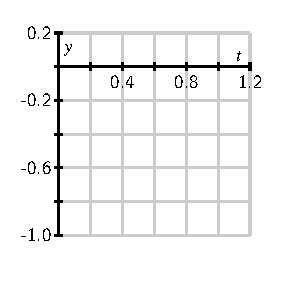
\includegraphics{figures/7_3_euler_empty.eps}}

\item Find the exact solution to the original initial value problem
  and use this function to find the error in your approximation at each one of the points
  $t_i$.

\item Explain why the value $y_5$ generated by Euler's method for this initial value problem
  produces the same value as a left Riemann sum for the definite integral $\int_0^1
  (2t-1)~dt$.  

\item How would your computations differ if the initial value was $y(0) =
  1$?  What does this mean about different solutions to this
  differential equation?   

\ea
\end{activity}
\begin{smallhint}
\ba
	\item Small hints for each of the prompts above.
\ea
\end{smallhint}
\begin{bighint}
\ba
	\item Big hints for each of the prompts above.
\ea
\end{bighint}
\begin{activitySolution}
\ba
	\item Solutions for each of the prompts above.
\ea
\end{activitySolution}
\aftera